\documentclass[12pt]{article}
\usepackage[top=1in,bottom=1in,left=1in,right=1in]{geometry}
\usepackage{alltt}
\usepackage{array}	
\usepackage{graphicx}
\usepackage{tabularx}
\usepackage{verbatim}
\usepackage{setspace}
\usepackage{listings}
\usepackage{amssymb,amsmath, amsthm}

\title{SOEN331: Introduction to Formal Methods\\for Software Engineering\\
Assignment 2 on Extended Finite State Machines}
\author{\begin{tabular}{c}
Alec Adub (40032876) \tabularnewline
Alex Frappier Lachapelle (40019133) \tabularnewline
Robert Nittolo (40032587) \tabularnewline
Pierre-Olivier Trottier (40059235) \tabularnewline\\
\end{tabular}
}
\date{\today}

\begin{document}
\begin{spacing}{1.5}

\maketitle

\newpage

\section{Formal specification}

\noindent \textbf{autonomous car}

\noindent The EFSM of the autonomous car is the tuple $S = (Q, \Sigma_1, \Sigma_2, q_0, V, \Lambda)$, where\\

\noindent $Q = \{idle, parked~mode, manual~ driving~mode, cruise~mode, panic~mode\}$\\
\noindent $\Sigma_1 = \{ignition, cruise, drive, switch~to~manual, turn~OFF~panic, unforseen~event, turn~OFF\}$\\
\noindent $\Sigma_2 = \{beep, car~is~stopped,  hazard~signal~is~turned~ON, hazard~signal~is~turned~OFF\}$\\
\noindent $q_0: idle$\\
\noindent $V: destination = \{is~set, is~not~ set\}~engine = \{is~idle, is~not~idle\}$\\
\noindent $\Lambda$: Transition specifications\\
\indent 1. $\rightarrow idle$\\
\indent 2. $parked~mode \xrightarrow {\text { cruise~[destination~is~set]}} cruise~mode$\\
\indent 3. $parked~mode \xrightarrow {\text { cruise~[destination~is~not~set]}} manual~driving~mode$\\
\indent 4. $parked~mode \xrightarrow {\text { drive~[engine~is~idle]}} manual~driving~mode$\\
\indent 5. $cruise~mode \xrightarrow {\text { drive~[engine~is~idle]}} parked~mode$\\
\indent 6. $cruise~mode \xrightarrow {\text { unforseen~event/car~is~stopped;~hazard~signal~is~turned~ON}} panic~mode$\\
\indent 7. $cruise~mode \xrightarrow {\text { switch~to~manual}} manual~mode$\\
\indent 8. $manual~driving~mode \rightarrow  parked~mode$\\
\indent 9. $parked~mode \rightarrow   turned~OFF$\\


\noindent The UML state diagram is shown in Figure~\ref{fig:state-diagram}.

\newpage

\section{UML state diagrams}

\begin{figure}[h!]
	\centering
		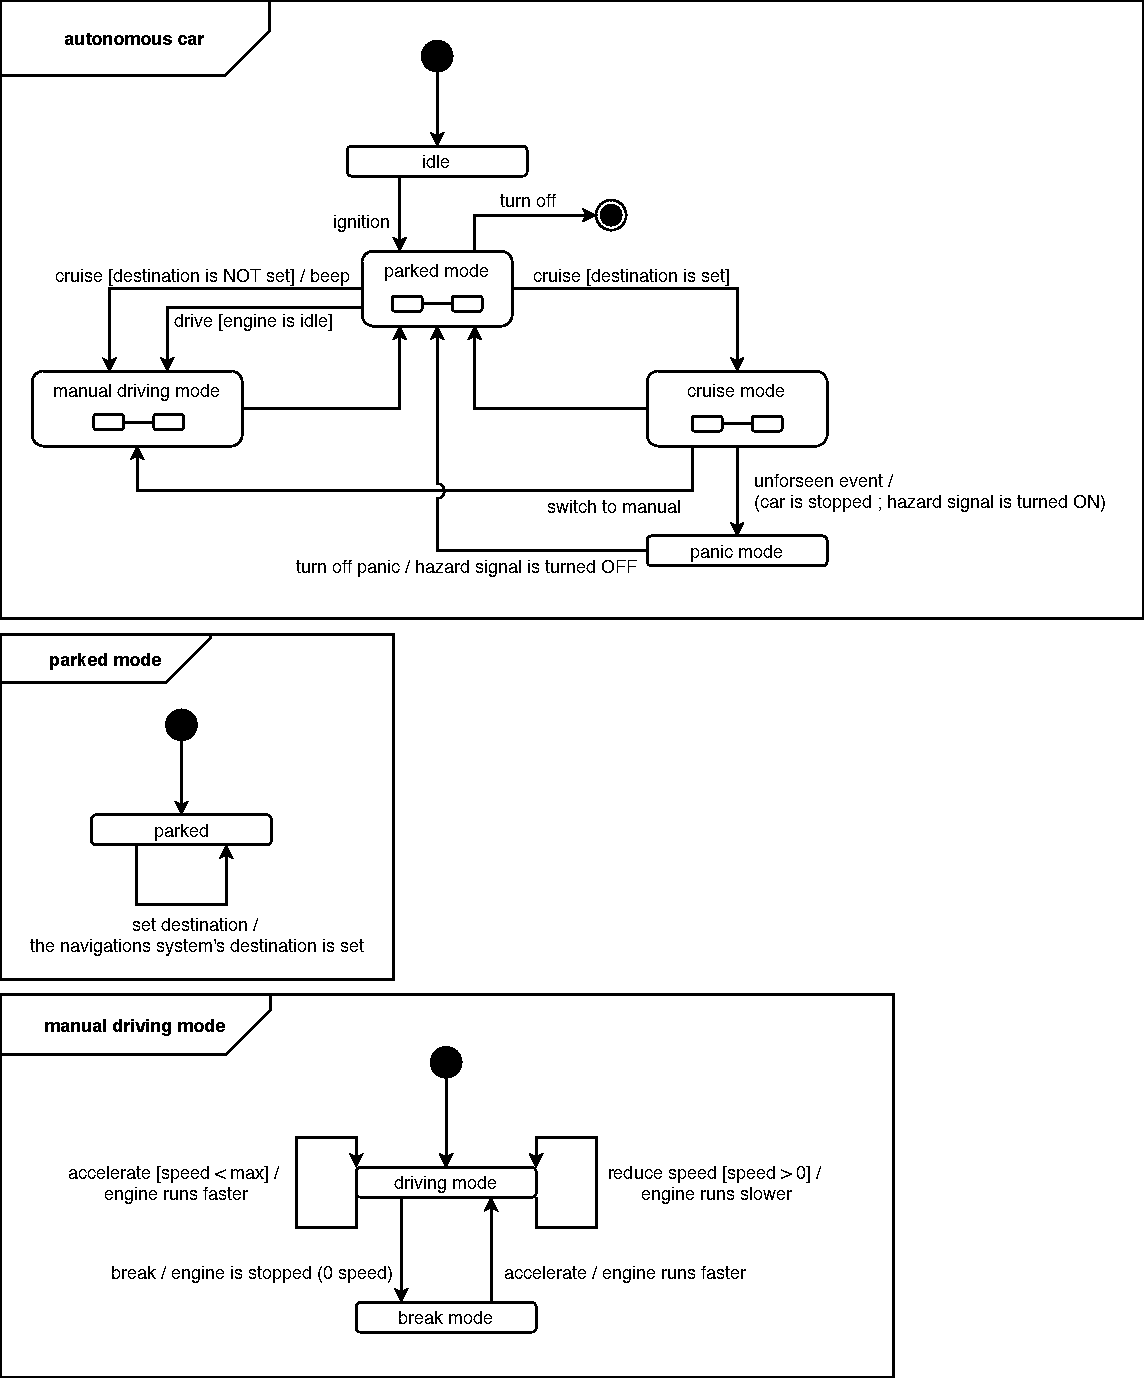
\includegraphics[width=1\textwidth]{./figures/eps/EFSM.eps}
		  \caption{UML state diagram of the autonomous car}
  \label{fig:state-diagram}
\end{figure}
\begin{figure}[h!]
	\centering
		\includegraphics[width=1\textwidth]{./figures/CruiseMode-p2}
		  \caption{UML state diagram of the autonomous car}
  \label{fig:state-diagram}
\end{figure}
\begin{figure}[h!]
	\centering
		\includegraphics[width=1\textwidth]{./figures/CruiseMode-p3}
		  \caption{UML state diagram of the autonomous car}
  \label{fig:state-diagram}
\end{figure}

\end{spacing}


\end{document}
